\documentclass[10pt, a4paper]{extarticle}
\usepackage[T1]{fontenc}
\usepackage[english]{babel}
\usepackage[margin=1cm]{geometry}
\usepackage[utf8]{inputenc}
\usepackage{fontawesome}
\usepackage{graphicx}
\usepackage{hyperref}
\usepackage{natbib}
\usepackage{microtype}
% List spacing
\usepackage{enumitem}
% Source Sans Pro font
\usepackage{sourcesanspro}
\renewcommand{\familydefault}{\sfdefault}
% Headings format 
\usepackage{titlesec}

\renewcommand{\bibsection}{\section*{Publications}}
\bibliographystyle{plainnat}
% Disable page number
\pagenumbering{gobble}


% Paragraph spacing
\usepackage{parskip}
% Headings

\titleformat*{\section}{\normalfont\large\bfseries}%\color{MidnightBlue}}

\titleformat*{\subsection}{\bfseries}%\color{MidnightBlue}}
% Title format
\makeatletter
\def\@maketitle{
  \newpage
  {\LARGE\textbf{{\@title}} \par}

  May 4th, 1998 | \faMapMarker ~ Bologna, Italy

  \href{mailto:kmfrick98@gmail.com}{\texttt{kmfrick98@gmail.com}}  | \url{https://kmfrick.tech}

  \url{https://github.com/kmfrick} | \url{https://linkedin.com/in/kmfrick}
  \hfill\smash{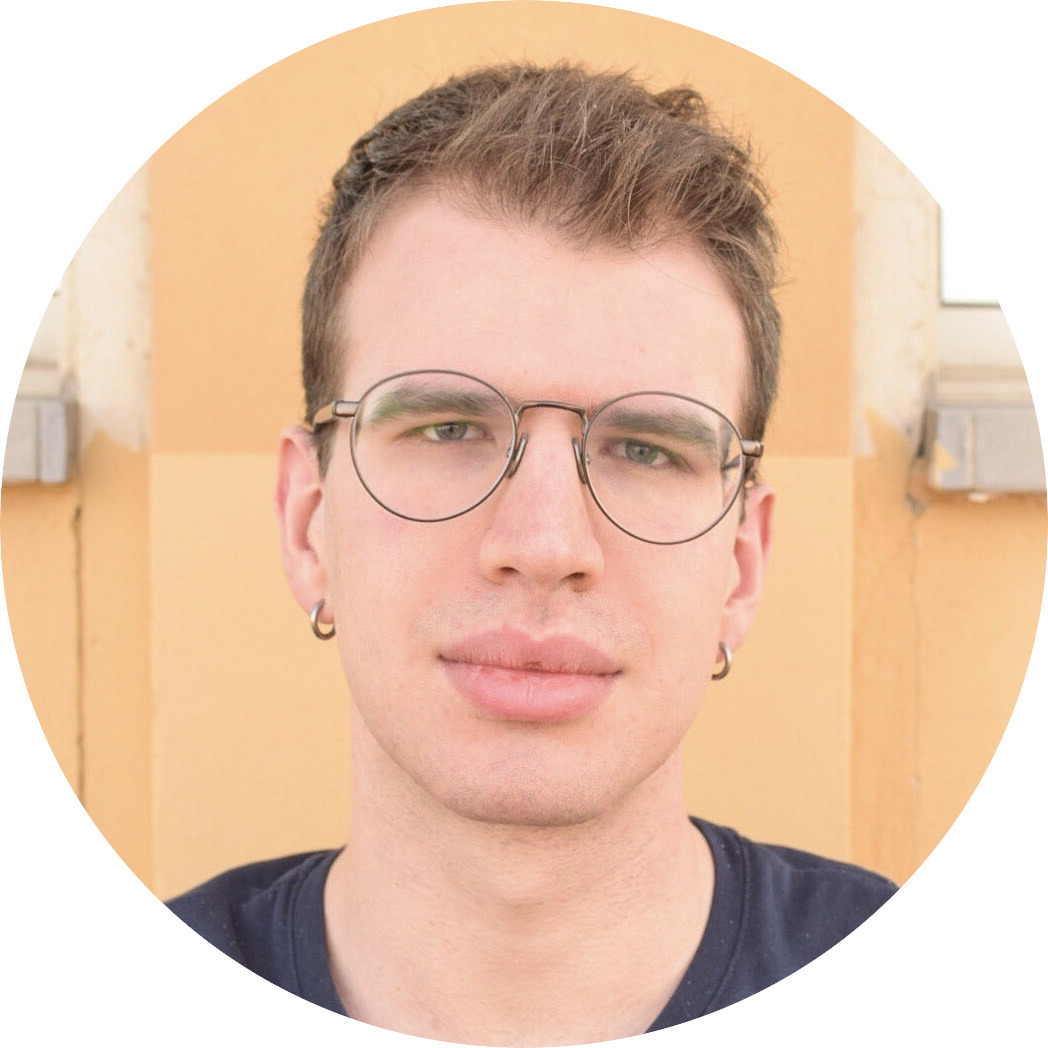
\includegraphics[width=3cm]{frickkm.JPG}}

  }
  \makeatother
  % Headings spacing 

  \titlespacing\section{0pt}{2pt plus 2pt minus 2pt}{2pt plus 2pt minus 2pt}

  \titlespacing\subsection{0pt}{2pt plus 2pt minus 2pt}{2pt plus 2pt minus 2pt}
  % List spacing
  \setlist{nosep, leftmargin=*}
  \setlist{parsep=1pt, topsep=1pt, itemsep=1pt, leftmargin=*}
  \title{Kevin Michael Frick}
  \author{}
  \begin{document}


  \maketitle
  \vspace{-0.8em}
  \hrulefill

  \section*{Work experience}
  \textbf{Computer Vision Research Intern} \hfill Robotics and Mechatronics, University of Twente, NL | 03/2020 - 06/2020

  \begin{itemize}
    \item Erasmus+ traineeship with the goal of improving the localization and mapping (SLAM) capabilities of an unmanned aerial vehicle through research and deployment of deep neural networks for semantic segmentation of 3D scenes
    \item Developed a module for the ROS framework able to integrate a state-of-the-art SLAM solution with neural networks that make use of TensorFlow's, TensorFlow Lite's and PyTorch's C++ and Python APIs
    \item Developed and deployed a Docker container that significantly reduced environment set-up times and compatibility issues
  \end{itemize}

  \section*{Education}

  \textbf{MSc Computer Engineering} \hfill Collegio Superiore, University of Bologna, IT | 09/2020 - Present
  \begin{itemize}
    \item Honors program of the University of Bologna, offering advanced and interdisciplinary education by means of courses, seminaries and lectures concerning various topics from different fields. 
    \item Admission depends on a selective test which is solely based on merit
    \item Seven BSc STEM students are admitted each year and are provided with a personal tutor, exemption from annual fees, free accommodation and an annual scholarship throughout their bachelor's and master's degrees
    \item Student representative to the Network of Italian Students in Schools and Institutes for Higher Study (RIASISSU) from 2020 to 2022. Responsible for organizing and coordinating joint activities between the Collegio Superiore and other Italian honors colleges
    \item Erasmus+ exchange at the Universitat Politècnica de Catalunya, Barcelona for the entire second year, with a study plan focused on reinforcement learning and algorithmic game theory

  \end{itemize}
  \textbf{BSc Computer Engineering} \hfill Collegio Superiore, University of Bologna, IT | 09/2017 - 07/2020 | Summa Cum Laude, GPA: 29.6/30
  \begin{itemize}
    \item Thesis: "Machine Learning for Semantic Visual SLAM"
    \item Acquired skills in programming, software engineering patterns and principles, statistical modeling, computer networks, database design, electronics and telecommunications
  \end{itemize}

  \section*{Languages}

  Italian, native speaker | English, CEFR C2, IELTS Academic 8.5 | Spanish, CEFR B2 university certification


  \section*{Projects, honors and awards}
  \begin{itemize}
    \item Led a team of 4 people to develop an \textbf{artificial intelligence} able to play the Nordic board game Tablut using informed tree search techniques, training metaparameters with a genetic algorithm
    \item Academic \textbf{digital systems} project: developed a parallelized implementation of the \textbf{Q-learning} algorithm leveraging \textbf{Xilinx FPGA} hardware using high-level synthesis tools
    \item One of 6 students selected to compete in the national final of the the \textbf{CyberChallenge.IT}, specializing in software security and reverse engineering challenges as well as system administration.
      Attended the local training program, an advanced course in cybersecurity alternating theoretical lessons and exercises on various topics such as cryptography, malware analysis, and web security, only available to students who pass both a general logic test and a programming test
    \item Game engine pathfinder: developed a \textbf{pathfinding solution} that is able to efficiently find optimal and collision-free paths for an arbitrary number of actors in an \textbf{open source reimplementation of a game engine}. Languages and libraries involved: C++11, Python 3, SDL, OpenAL
    \item Academic \textbf{software engineering} project: led a team of 3 people to detail an in-depth requirements, domain and risk analysis and develop a software solution to manage a bike rental service. Personally designed mock-ups of the UI using Figma. Languages and frameworks involved: Azure App Service, C\# 8.0, .NET Core 3.1, Azure SQL, Entity Framework Core, Bootstrap 4, jQuery
    \item OrarioSync: \textbf{web application} that allows users to download their college timetables and allow for phone calendar synchronization. Languages and frameworks involved: Python 3, ZEIT Now v2, JavaScript ES6, React
    \item Italian national selection for the International Olympiad in Informatics (IOI): \textbf{bronze medal} won in the 2016 final round of individual competitions, \textbf{third place} in the 2016 final round of team competitions


  \end{itemize}

  \section*{Teaching activities}


  \subsection*{Bachelor's}
  \begin{itemize}

    \item Software Engineering | Teaching Assistant \hfill University of Bologna, 2021

  \end{itemize}

  \subsection*{High school}
  \begin{itemize}

    \item Competitive Programming | Teacher \hfill Istituto Tecnico Aldini Valeriani, Bologna, 2020-2021

    \item Computer Science | Teacher \hfill  Istituto Tecnico Aldini Valeriani, Bologna, 2020-2021
  \end{itemize}
  \nocite{*}
  \bibliography{CV}
\end{document}
